\section{Testmiljø}
I dette afsnit præsenteres testmiljøet der sat op til at teste robottens færdigheder.

\subsection{Formål}
Formålet med et testmiljø er for bedre at kunne kontrollere omgivelserne.
Dette giver mindre unøjagtigheder ifht. hvis det skulle testes i et nyt miljø hver gang og muligheden for at sammenligne resultater.

\subsection{Opsætning}\label{testmiljo:opsaetning}
Testmiljøet er opsat vha. papkasser og tape, som man kan se på \cref{testmiljo:perspektiv}.
Størrelsen er $189 \ cm \times 261 \ cm$ grunden til denne størrelse er at dette præcis passer ifht. kinectens billede som man kan se på \cref{testmiljo:oppefra}.
På \cref{testmiljo:forfra} kan man se hvordan kinecten er monteret under en loftplade.

\begin{figure}
\begin{tikzpicture}
\node[anchor=south west,inner sep=0] at (0,0) {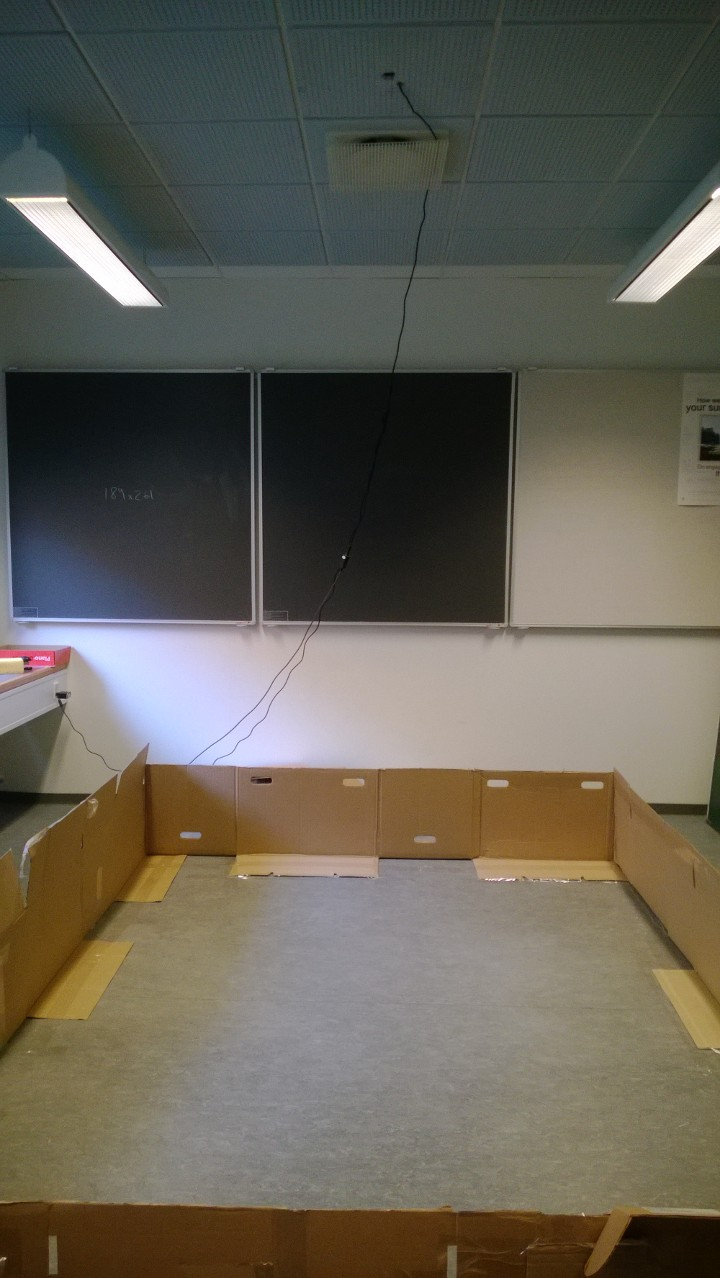
\includegraphics[width=\textwidth/2]{./verden/forfra}};
    \draw [->, red, ultra thick] (5.5,10.5) -- (4.2,11.2);
\end{tikzpicture}
\caption{Testmiljøet set forfra. Bemærk kinecten monteret i en loftplade(rød pil) med hul til RGB-kameraet.}
\label{testmiljo:forfra}
\end{figure}

\begin{figure}
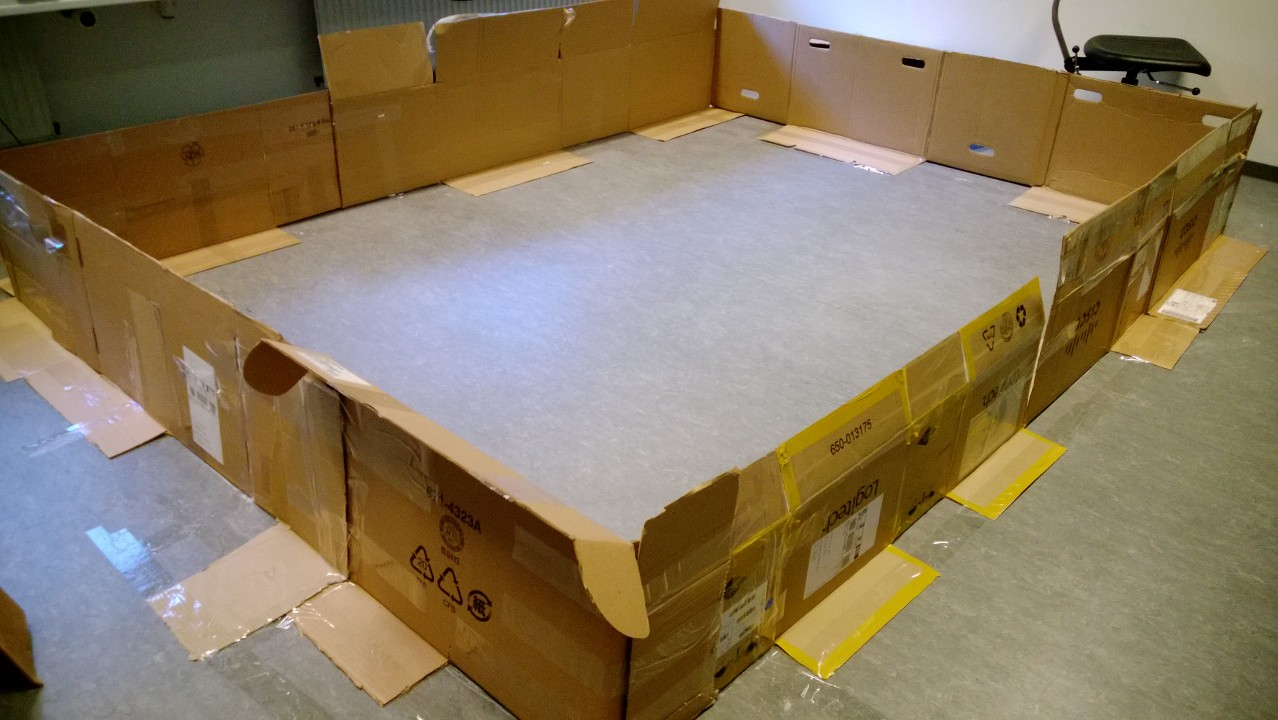
\includegraphics[width=\textwidth]{./verden/perspektiv}
\caption{Testmiljøet set i perspektiv.}
\label{testmiljo:perspektiv}
\end{figure}

\begin{figure}
\begin{tikzpicture}
\node[anchor=south west,inner sep=0] at (0,0) {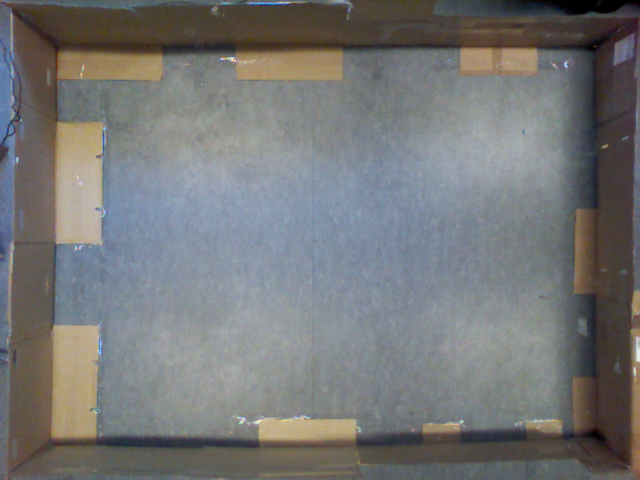
\includegraphics{./verden/oppefra}};
    \draw [<->, red, ultra thick] (1.3,0.9) -- (1.5,11.4);
    \node [red, ultra thick] at (2.5,5.5) {189 cm};
    \draw [<->, red, ultra thick] (1.3,0.9) -- (16,1);
    \node [red, ultra thick] at (8, 2) {261 cm};
\end{tikzpicture}
\caption{Testmiljøet set fra kinecten.}
\label{testmiljo:oppefra}
\end{figure}